\section{Chopping and reassembly}\label{s:chop}

\begin{figure*}[t!]%
\definecolor{hair}{gray}{1}%
\definecolor{head}{rgb}{.85,.85,1}%
\definecolor{body}{rgb}{.5,.8,.5}%
\definecolor{tail}{rgb}{.55,.55,.55}%
\centering
\begin{subfigure}[t]{.475\linewidth}
\centering
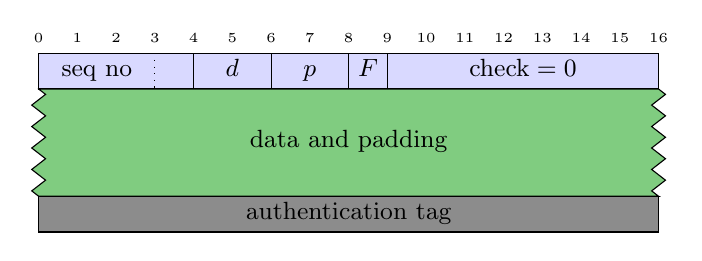
\begin{tikzpicture}[x=1.75pt,y=3ex]
\small
{\tiny
\foreach \x/\l in {0/0, 8/1, 16/2, 24/3, 32/4, 40/5, 48/6, 56/7,
                   64/8, 72/9, 80/10, 88/11, 96/12, 104/13, 112/14,
                   120/15, 128/16}
  \node [above] at (\x,0.1) {\l} ;
}
\filldraw [fill=head] (0,0) rectangle (128,-1) ;
\draw (32,0) -- (32,-1)
      (48,0) -- (48,-1)
      (64,0) -- (64,-1)
      (72,0) -- (72,-1) ;
\draw [dotted] (24, 0) -- (24, -1) ;
\node [anchor=mid,inner sep=0pt, outer sep=0pt] at (12,  -0.5) {seq no} ;
\node [anchor=mid,inner sep=0pt, outer sep=0pt] at (40,  -0.5) {$d$} ;
\node [anchor=mid,inner sep=0pt, outer sep=0pt] at (56,  -0.5) {$p$} ;
\node [anchor=mid,inner sep=0pt, outer sep=0pt] at (68,  -0.5) {$F$} ;
\node [anchor=mid,inner sep=0pt, outer sep=0pt] at (100, -0.5)
   {$\mbox{check} = 0$} ;
\filldraw [fill=body,decoration={zigzag,segment length=2ex}]
  (128,-1) decorate { -- (128,-4) } -- (0,-4) decorate { -- (0,-1) } -- cycle;
\node [anchor=mid,inner sep=0pt, outer sep=0pt] at (64,-2.5)
  {data and padding} ;
\filldraw [fill=tail] (0,-4) rectangle (128,-5) ;
\node [anchor=mid,inner sep=0pt, outer sep=0pt] at (64,-4.5)
  {authentication tag} ;
\end{tikzpicture}%
\caption{Blocks consist of a header, up to $2^{15}-1$ bytes each of
  data and padding, and an authentication tag. $d$:~data length;
  $p$:~padding length; $F$:~function code.  $d+p$ is not required to
  be a multiple of 16.\label{f:block}}
\end{subfigure}
\quad
\begin{subfigure}[t]{.47\linewidth}
\centering
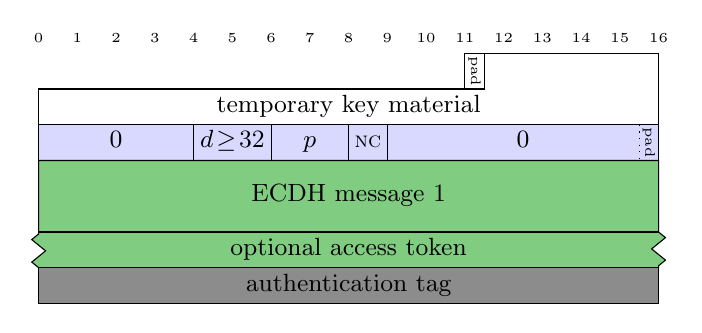
\begin{tikzpicture}[x=1.75pt,y=3ex]
\small
{\tiny
\foreach \x/\l in {0/0, 8/1, 16/2, 24/3, 32/4, 40/5, 48/6, 56/7,
                   64/8, 72/9, 80/10, 88/11, 96/12, 104/13, 112/14,
                   120/15, 128/16}
  \node [above] at (\x,2.1) {\l} ;
}
\filldraw [fill=hair] (0,1) -- (0,0) -- (128,0) -- (128,2)
                            -- (88,2) -- (88,1) -- cycle;
\draw (88,1) -- (92,1) -- (92,2) ;
\node [rotate=-90] at (90,  1.5) {\tiny pad};
\node [anchor=mid,inner sep=0pt, outer sep=0pt] at (64,0.5)
 {temporary key material};
\filldraw [fill=head] (0,0) rectangle (128,-1) ;
\draw (32,0) -- (32,-1)
      (48,0) -- (48,-1)
      (64,0) -- (64,-1)
      (72,0) -- (72,-1) ;
\draw [dotted] (124,0) -- (124,-1) ;
\node [anchor=mid,inner sep=0pt, outer sep=0pt] at (16,  -0.5) {0} ;
\node [anchor=mid,inner sep=0pt, outer sep=0pt] at (40,  -0.5) {$d\!\ge\!32$} ;
\node [anchor=mid,inner sep=0pt, outer sep=0pt] at (56,  -0.5) {$p$} ;
\node [anchor=mid,inner sep=0pt, outer sep=0pt] at (68,  -0.5)
  {\footnotesize\scshape nc} ;
\node [anchor=mid,inner sep=0pt, outer sep=0pt] at (100, -0.5) {0} ;
\node [rotate=-90] at (126, -0.5) {\tiny pad};
\filldraw [fill=body,decoration={zigzag,segment length=2.1ex}]
    (0,-1) -- (128,-1) -- (128,-3) decorate { -- (128,-4) }
    -- (0,-4) decorate { -- (0,-3) } -- cycle;
\node [anchor=mid,inner sep=0pt, outer sep=0pt]
  at (64,-2) {ECDH message 1};
\node [anchor=mid,inner sep=0pt, outer sep=0pt]
  at (64,-3.5) {optional access token};
\draw (0,-3) -- (128,-3) ;
\filldraw [fill=tail] (0,-4) rectangle (128,-5) ;
\node at (64,-4.5) {authentication tag} ;
\end{tikzpicture}
\caption{A new-link request consists of a Möller key encapsulation,
  followed by a block encrypted with the temporary key material.  Four
  padding bits are copied into the “check” field to make them
  non-malleable.\label{f:cnewlink}}
\end{subfigure}
\quad
\begin{subfigure}[t]{.47\linewidth}
\centering
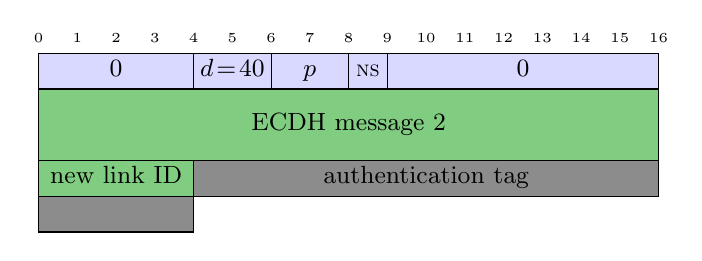
\begin{tikzpicture}[x=1.75pt,y=3ex]
\small
{\tiny
\foreach \x/\l in {0/0, 8/1, 16/2, 24/3, 32/4, 40/5, 48/6, 56/7,
                   64/8, 72/9, 80/10, 88/11, 96/12, 104/13, 112/14,
                   120/15, 128/16}
  \node [above] at (\x,0.1) {\l} ;
}
\filldraw [fill=head] (0,0) rectangle (128,-1) ;
\draw (32,0) -- (32,-1)
      (48,0) -- (48,-1)
      (64,0) -- (64,-1)
      (72,0) -- (72,-1) ;
\node [anchor=mid,inner sep=0pt, outer sep=0pt] at (16,  -0.5) {0} ;
\node [anchor=mid,inner sep=0pt, outer sep=0pt] at (40,  -0.5) {$d\!=\!40$} ;
\node [anchor=mid,inner sep=0pt, outer sep=0pt] at (56,  -0.5) {$p$} ;
\node [anchor=mid,inner sep=0pt, outer sep=0pt] at (68,  -0.5)
  {\footnotesize\scshape ns} ;
\node [anchor=mid,inner sep=0pt, outer sep=0pt] at (100, -0.5) {0} ;
\fill [fill=body] (0,-1) -- (128,-1) -- (128,-3) -- (32,-3) -- (32,-4)
               -- (0,-4) -- cycle;
\fill [fill=tail] (32,-3) rectangle (128,-4) (0,-4) rectangle (32,-5) ;
\draw (0,-1) rectangle (128,-3)
      (0,-3) rectangle (128,-4)
      (0,-4) -- (0,-5) -- (32,-5) -- (32,-3) ;
\node [anchor=mid,inner sep=0pt, outer sep=0pt] at (64,-2)
  {ECDH message 2};
\node [anchor=mid,inner sep=0pt, outer sep=0pt] at (16,-3.5) {new link ID};
\node [anchor=mid,inner sep=0pt, outer sep=0pt] at (80,-3.5)
  {authentication tag} ;
\end{tikzpicture}
\caption{A new-link response is a normal block, encrypted with the
  temporary key material.\label{f:snewlink}}
\end{subfigure}
\quad
\begin{subfigure}[t]{.475\linewidth}
\centering
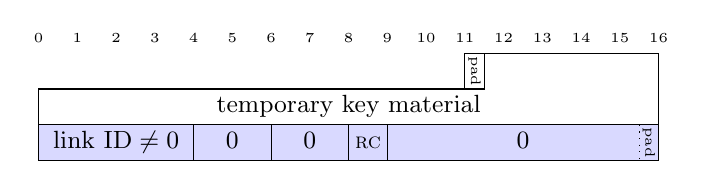
\begin{tikzpicture}[x=1.75pt,y=3ex]
\small
{\tiny
\foreach \x/\l in {0/0, 8/1, 16/2, 24/3, 32/4, 40/5, 48/6, 56/7,
                   64/8, 72/9, 80/10, 88/11, 96/12, 104/13, 112/14,
                   120/15, 128/16}
  \node [above] at (\x,2.1) {\l} ;
}
\filldraw [fill=hair] (0,1) -- (0,0) -- (128,0) -- (128,2)
                            -- (88,2) -- (88,1) -- cycle;
\draw (88,1) -- (92,1) -- (92,2) ;
\node [rotate=-90] at (90,  1.5) {\tiny pad};
\node [anchor=mid,inner sep=0pt, outer sep=0pt] at (64,0.5)
 {temporary key material};
\filldraw [fill=head] (0,0) rectangle (128,-1) ;
\draw (32,0) -- (32,-1)
      (48,0) -- (48,-1)
      (64,0) -- (64,-1)
      (72,0) -- (72,-1) ;
\draw [dotted] (124,0) -- (124,-1) ;
\node [anchor=mid,inner sep=0pt, outer sep=0pt] at (16,  -0.5)
  {$\mbox{link ID} \ne 0$} ;
\node [anchor=mid,inner sep=0pt, outer sep=0pt] at (40,  -0.5) {0} ;
\node [anchor=mid,inner sep=0pt, outer sep=0pt] at (56,  -0.5) {0} ;
\node [anchor=mid,inner sep=0pt, outer sep=0pt] at (68,  -0.5)
  {{\footnotesize\scshape rc}} ;
\node [anchor=mid,inner sep=0pt, outer sep=0pt] at (100, -0.5) {0} ;
\node [rotate=-90] at (126, -0.5) {\tiny pad};
\end{tikzpicture}%
\caption{A reconnection request is just a key encapsulation and a
  modified header. The link ID replaces the sequence number, $d$ and
  $p$ must be zero, and there is no authentication tag.\label{f:creconn}}
\end{subfigure}
\caption{Message formats before steganography.  Background shading
  indicates encryption mode.  {\color{head}$\blacksquare$}:~header
  encryption; {\color{body}$\blacksquare$}:~GCM encryption;
  {\color{tail}$\blacksquare$}:~GCM authentication tag;
  {$\square$}:~Möller key encapsulation.  There are 16 bytes per row
  of each diagram.\label{f:msgfmt}}
\end{figure*}


As we described briefly in Section~\ref{s:arch}, chopping converts the
traffic on a Tor link into a more malleable format: a sequence of
variable-size \emph{blocks}, independently padded and deliverable out
of order.  Every byte of each block is computationally
indistinguishable from randomness, as defined in~\cite{s-noncephil};
this is a baseline requirement for the hiddentext in theoretically
secure steganographic schemes.~\cite{s-ah-pssteg,s-ah-pksteg}  The
module that performs this job (and its inverse) is, naturally, called
the \emph{chopper}.

The block format is shown in Figure~\ref{f:block}.  The bulk of each
block is encrypted using AES in GCM mode~\cite{s-gcm}, which provides
both confidentiality and message integrity~\cite{s-authenc}.  The
block header consists of a 32-bit sequence number; two length fields,
$d$ and $p$, indicating respectively how much data and padding the
block carries; an opcode field, $F$, discussed below; and a 56-bit
check field, which must be zero.  The minimum block length is $32$
bytes ($128$-bit header, $128$-bit MAC) and the maximum is $2^{17} +
32$ bytes.  Block length is controlled by the steganography modules;
the chopper will fabricate blocks exactly as long as requested, using
data if possible, padding if there is not enough.  Padding consists of
binary zeroes.  Blocks containing only padding ($d=0$) are generated
when there is no data available but the cover protocol requires
transmission.

The sequence number permits the receiver to sort incoming blocks into
their original order.  It serves the same function as a TCP sequence
number, but it always starts at zero, counts blocks rather than bytes,
and may not wrap around (see Section~\ref{s:rekey}).  It also serves
to ensure that the same header is never transmitted twice.  This is
important because the header must also be encrypted to render it
indistinguishable from randomness, and needs integrity protection to
preclude chosen-ciphertext attacks~\cite{a-padding-oracle,a-ssh-plaintext},
but we can't include it in the data authenticated by GCM because we
have to decrypt $d$ and $p$ in order to know where the authentication
tag begins.

Instead, we protect the header with a custom short-message
authenticated encryption mode that relies only on the basic AES
pseudorandom permutation.  The check field brings the header up to
exactly the AES block size, and we encrypt it as a standalone block
with a different key from that used for the payload.  Before the
receiver acts on a decrypted header, it verifies that every bit of the
check field is zero, and that the sequence number is within a
256-block-wide receive window.  An active attacker who modifies the
ciphertext of the header has less than one chance in $2^{80}$ of
passing this verification.  We recycle the \emph{ciphertext} of the
header as the GCM nonce for the payload.

\subsection{Function Codes}\label{s:f-codes}

The $F$ field of the block header controls how the receiver will
process the block. All presently-defined codes are listed in
Table~\ref{t:fcodes}.  Some codes are only valid in handshakes; see
below.

\begin{table}[h!]
\begin{tabular}{rlp{.70\columnwidth}}
\toprule
\textbf{No.} & \textbf{Name} & \textbf{Semantics} \\
\midrule
0   & \textsc{data} & Application data to be relayed.\\
1   & \textsc{fin}  & Last block of application data to be relayed.\\
2   & \textsc{rst}  & Protocol error; close the link immediately.\\
3   & \textsc{rc}   & Reconnect: associate this new connection with an
                      existing link.\\
4   & \textsc{nc}   & New link, client side.
                      See section~\ref{s:handshake} for details.\\
5   & \textsc{ns}   & New link, server side.\\
6   & \textsc{rki}  & Initiate rekeying; see
                      Section~\ref{s:rekey} for details.\\
7   & \textsc{rkr}  & Respond to rekeying.\\
8\rlap{--127}&      & Reserved for future definition.\\
128\rlap{--255}&    & Reserved for steganography modules.\\
\bottomrule
\end{tabular}
\caption{Codes for the $F$ field}\label{t:fcodes}
\end{table}

\subsection{Handshake Messages}\label{s:handshake}

The first few bytes of data sent on each new connection are a
\emph{handshake message} (henceforth just “handshake”), which informs
the server whether this connection belongs to an existing link or to a
new one.  If the connection belongs to a new link, the server replies
with a handshake of its own, and both peers derive new session keys
for the link from the data in the handshakes.  There are three
handshake formats, shown in figures~\ref{f:cnewlink}, \ref{f:creconn},
and~\ref{f:snewlink}.  Handshakes have similar overall structure to
blocks, but vary in details.

Most asymmetric cryptosystems' ciphertexts are easily distinguished
from randomness. We use Möller's elliptic-curve key encapsulation
mechanism~\cite{s-moller}, which is designed to produce random
ciphertexts. It can only be used to establish a weak shared secret,
which we refer to as “temporary key material.”  It has the unfortunate
property of producing 164-\emph{bit} messages, which must be padded to
a whole number of bytes.  The padding bits could be flipped by an
adversary without any visible effect.  To prevent this information
leak, the \emph{check} field of the header that immediately follows a
key encapsulation contains a copy of the padding.  Also, the server
must maintain a replay cache of all key encapsulations it has seen
recently, and discard any handshake with a replayed encapsulation,
even if the data that follows is different.

Each link has a nonzero, 32-bit \emph{link ID}.  The server chooses
this ID during link setup, making sure that it is unique among all
active or recently-active connections to the same server.  It is never
transmitted in cleartext, so it need not be random.

Key derivation, whether from the temporary key material or from
Diffie-Hellman exchanges, is done with HKDF-SHA256~\cite{s-hkdf1},
salted with the server's public key, and produces four 128-bit AES
keys: server-to-client payload key, server-to-client header key,
client-to-server payload key, and client-to-server header key, in that
order.

\subsubsection{New Link Handshake}

Link setup is loosely based on the STS protocol~\cite{s-sts} and
provides forward secrecy.  Initially, the client knows the server's
public key.  It has no asymmetric keypair of its own, but it may have
an “access token” which will identify it to the server.  This token is
opaque to the client, and its contents are outside the scope of this
paper.

The client's first message to the server is shown in
figure~\ref{f:cnewlink}.  It begins with a randomly chosen Möller key
encapsulation, followed by a special block encrypted with the
temporary key material.  This block has sequence number 0, and its $F$
code is \textsc{rc}.  Its first 32 bytes are an ECDH message on the
NIST standard curve P-256~\cite{s-fips186-2}, derived from a source of
strong randomness.  Only the $x$-coordinate of the public point is
transmitted.  If the client has an access token, it follows
immediately after the ECDH message.

If the server can decrypt this handshake and finds the access token
(if any) acceptable, it replies with its own handshake, shown in
figure~\ref{f:snewlink}.  This is a normal block, also encrypted with
the temporary key material provided by the client.  It also has
sequence number 0, its $F$ code is \textsc{rs}, and its contents are
another ECDH message and the link ID for the new link.  Once the
client receives this message, both sides can complete the
Diffie-Hellman exchange and derive long-lived keys for the link.
Subsequent blocks are encrypted with those keys.  The handshakes count
as sequence number 0 in each direction.

\subsubsection{Reconnection Handshake}

For new connections to established links, the client's handshake needs
to be as short as possible.  It is shown in figure~\ref{f:creconn}.
As with a new-link handshake, it begins with a randomly chosen Möller
key encapsulation, but instead of a block, only a modified header
follows.  This header has $p=0$, $d=0$, and $F=\text{\textsc{rc}}$,
and it carries the desired link ID in place of the sequence number.
Unlike normal blocks with $p=0$ and $d=0$, the GCM authentication tag
is omitted.  The client may transmit blocks, encrypted with the
appropriate link keys, immediately after this handshake (that is, in
the same cover-protocol message).

\subsection{Rekeying}\label{s:rekey}

Rekeying is very similar to key derivation for a new link, but uses
blocks rather than special handshake messages.  Rekeying resets the
sequence number but does not change the link ID.  Either peer may
initiate a rekeying cycle at any time by transmitting an
\textsc{rki} block.  Peers are \emph{required} to rekey before the
sequence number wraps around, and encouraged to rekey considerably
sooner.

An \textsc{rki} block's data section is simply an ECDH message on curve
P-256.  The recipient of this message responds with an \textsc{rkr}
block, whose data section is another ECDH message.  Upon receipt of
\textsc{rkr}, both peers derive new link keys from the Diffie-Hellman
exchange, just as they would have for a new link.  It is a protocol
error to transmit any blocks after \textsc{rki} until receipt of
\textsc{rkr}, or to transmit blocks using the old keys after
transmitting \textsc{rkr}.

\subsection{Link Termination}

When both sides have sent and received a \textsc{fin} block, the link
is closed; however, both sides must remember the link ID for some
time, to guard against replay attacks or delayed block arrival.  It is
a protocol error to transmit a \textsc{data} block with a nonzero $d$
field after transmitting a \textsc{fin} block; however, \textsc{data}
blocks with $d=0$ may still be sent, and other function codes may be
used if appropriate.  For instance, the \textsc{rki} block requires a
response, even if the recipient has already transmitted a
\textsc{fin}.
